% ========================================================================
% ELEMENTOS PÓS-TEXTUAIS
% Referências, apêndices e anexos conforme ABNT NBR 14724:2011
% ========================================================================

% ========================================================================
% REFERÊNCIAS BIBLIOGRÁFICAS
% ========================================================================
\postextual

% Configura o título das referências
\bibliography{referencias}

% ========================================================================
% GLOSSÁRIO (OPCIONAL)
% ========================================================================
% Descomente se necessário incluir glossário
% \glossary

% ========================================================================
% APÊNDICES (OPCIONAL)
% ========================================================================
% Descomente e personalize se houver apêndices
% Os apêndices são textos elaborados pelo próprio autor

\begin{apendicesenv}
    % Imprime uma página indicando o início dos apêndices
    % \partapendices
    
    % ========================================================================
    % APÊNDICE A - EXEMPLO DE APÊNDICE
    % ========================================================================

    \begin{figure}[H]
        \textbf{APÊNDICE A – EXTRATOS DOS LOGS DE AUDITORIA DA API}
        \centering
        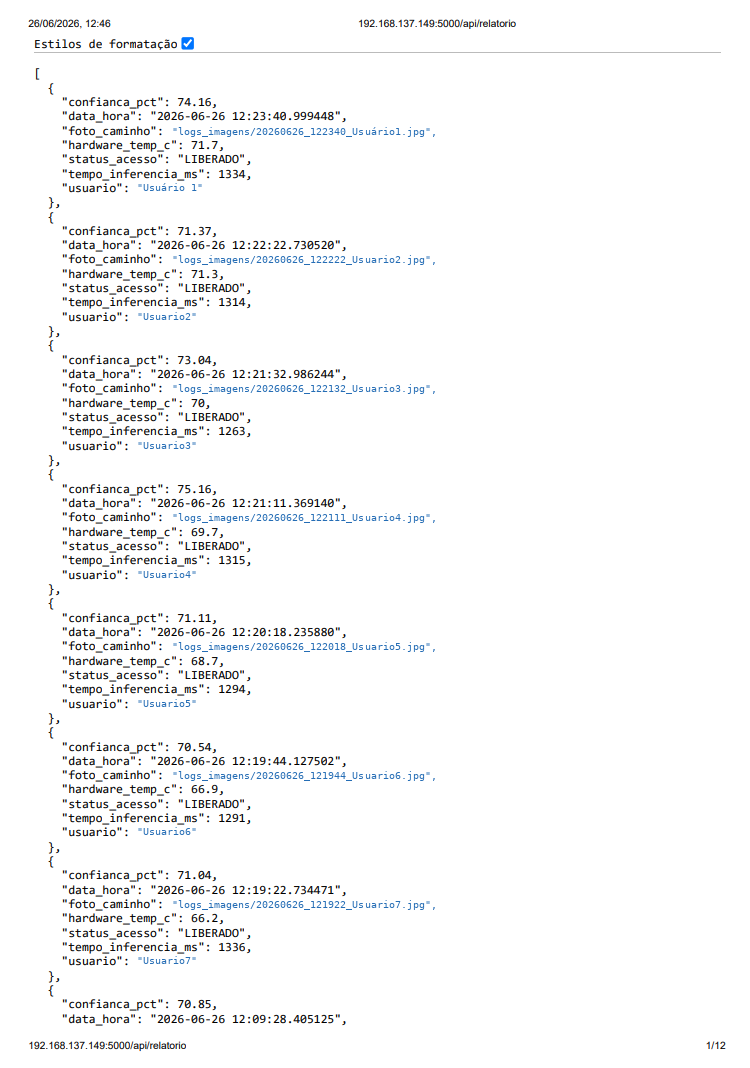
\includegraphics[width=1\textwidth]{img/apendice/folha de relatorio 1 (anonimizada).png} 
        \vspace{0.3em}
        \footnotesize 
        \label{fig:folha-relatorio1}
    \end{figure}
    \begin{figure}[H]
        \textbf{APÊNDICE B - REGISTRO BRUTO DE CRONOMETRAGEM DOS ATENDIMENTOS NAS CLÍNICAS AMOSTRADAS}
        \centering
        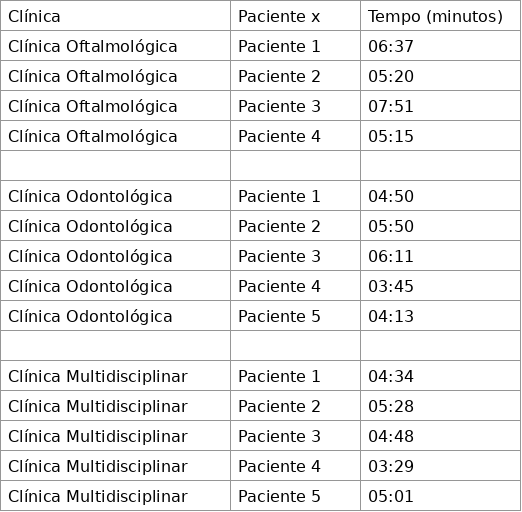
\includegraphics[width=1\textwidth]{img/apendice/tempo-conometrado.png} 
        \vspace{0.3em}
        \footnotesize 
        \label{fig:folha-relatorio1}
    \end{figure}
    \begin{figure}[H]
        \textbf{APÊNDICE C - EXTRATO DAS RESPOSTAS AO FORMULÁRIO DE MAPEAMENTO DE PROCESSOS}
        \centering
        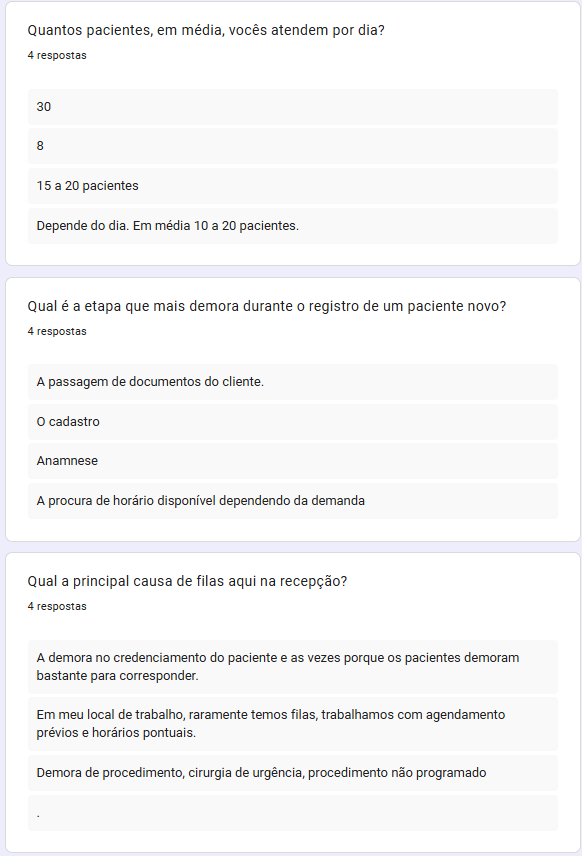
\includegraphics[width=1\textwidth]{img/apendice/mapeamento-processos1.png} 
        \vspace{0.3em}
        \footnotesize 
        \label{fig:folha-relatorio1}
    \end{figure}
    \begin{figure}[H]
        \centering
        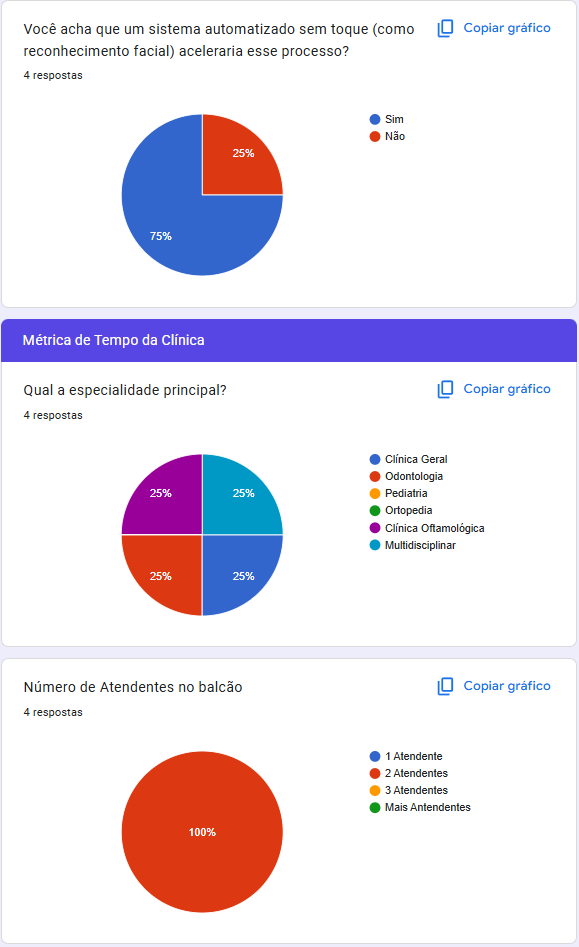
\includegraphics[width=1\textwidth]{img/apendice/mapeamento-processos2.png} 
        \vspace{0.3em}
        \footnotesize 
        \label{fig:folha-relatorio1}
    \end{figure}
    \begin{figure}[H]
        \centering
        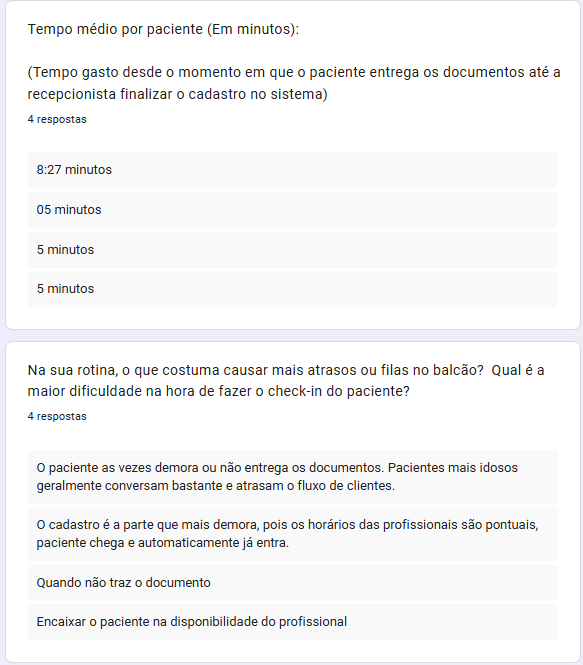
\includegraphics[width=1\textwidth]{img/apendice/mapeamento-processos3.png} 
        \vspace{0.3em}
        \footnotesize 
        \label{fig:folha-relatorio1}
    \end{figure}
    \textbf{APÊNDICE D - DOCUMENTAÇÃO DO PROJETO} \\
    \url{https://face-recognition-totem.netlify.app/#} \\
    \url{https://github.com/Victor-Sarris/Totem-Reconhecimento-Facial}
\end{apendicesenv}
